
\chapter{Improvements}
\section{More deadlock detection}
To improve the algorithm, better deadlock detections must be created. The first to implement would be heuristics that detect the states in figure \ref{fig:missingdeadlocks}.

First of all it should not be allowed to put two boxes into the same narrow corridor as you cannot get in between the boxes thus making the boxes deadlock. (The left image in figure \ref{fig:missingdeadlocks}.) One way of solving this could be to make the corridor a one box only zone and lock it as soon as a box is inside it.

Furthermore a deadlock detector that is able to check if a room with only one entrance is getting blocked, must be created. (The right image). There are many aspects in this: first of all how do you find areas with only one entrance? And how do you decide whther the entrance is blocked? And how do you do this without making the algorithm very slow?

\begin{figure}[htp]
	\centering
	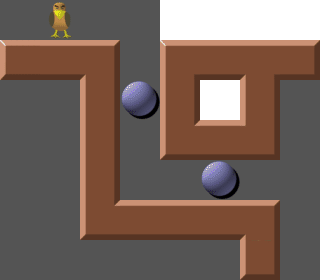
\includegraphics[width=0.4\textwidth]{blockednarrow}
	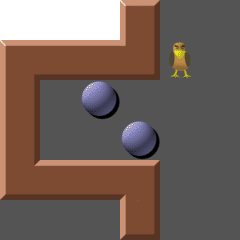
\includegraphics[width=0.4\textwidth]{blockedentrance}
	\caption{Deadlocks not found by our heuristics}
	\label{fig:missingdeadlocks}
\end{figure}
